%!TEX root = ../scivis_lbaakman_bvanloon.tex
\todo[inline]{Introduce the section}
In this section the main methods are given that are used to construct the colormaps.


\subsection{Texture Mapping} % (fold)
\label{sub:texture_mapping}
To implement the colormaps \emph{texture mapping} is used. The general pipeline of texture mapping is as follows.
\begin{enumerate}
	\item First the scalar values are sampled for each vertex in the simulation grid.
	\item Next the vertices of the triangulation of the simulation grid is passed to the vertex shader with the associated scalar values.
	\item The vertex shader normalizes scalar values associated with the vertices using a given range of the scalar values creating texture-coordinates for every vertex.
	\item The texture-coordinates are passed to the fragment shader and automatically interpolated by OpenGL.
	\item Next each fragment is rendered by the fragment shader, using the (interpolated) texture-coordinates to lookup the right texture (color) in the colormap.
\end{enumerate}
The end result is a piecewise-linear reconstruction of the (sampled) simulation values. By interpolating the texture coordinates, interpolation of colors is prevented.  This means that no false colors are displayed in the visualization. This is also the main motivation for the choice of texture mapping. The alternative (naive) method of vertex-based colormapping can result in colors that do not correspond with the actual scalar values or even worse, colors that are not in the colormap. These problems are prevented by using texture-based colormapping resulting in a true representation of the scalar values for every pixel.

By using texture mapping a colormap can be generated by constructing a 1D texture that represents the range of colors that are associated with the normalized scalar values. By using the normalized scalar value as index of this 1D texture the corresponding color can be retrieved. By using this approach a colormap can be added to the visualization by providing its 1D texture.

\subsection{Parameterization of Color Maps}
\label{ss:colormaps:parameterization}
There are a few parameters that are of importance which can influence the colormap design. The first parameters is the number of colors used in the colormap. When the number of colors is low there is a relatively large difference between two neighboring colors in the colormap. This large step will also be present in the visualization causing sharp edges between areas with different scalar values. An example of the banding effect is given in figure \ref{fig:colormaps:banding} which shows the difference between two colormaps that uses the same color-scheme with one containing 20 colors and the second containing 256 colors. Here we can see that \cref{fig:colormapping:banding:20} shows distinct bands, while \cref{fig:colormapping:banding:256} appear to have smooth transactions between the colors.
\begin{figure}[tb]
	\centering
	\begin{subfigure}{0.4\textwidth}
		\centering
		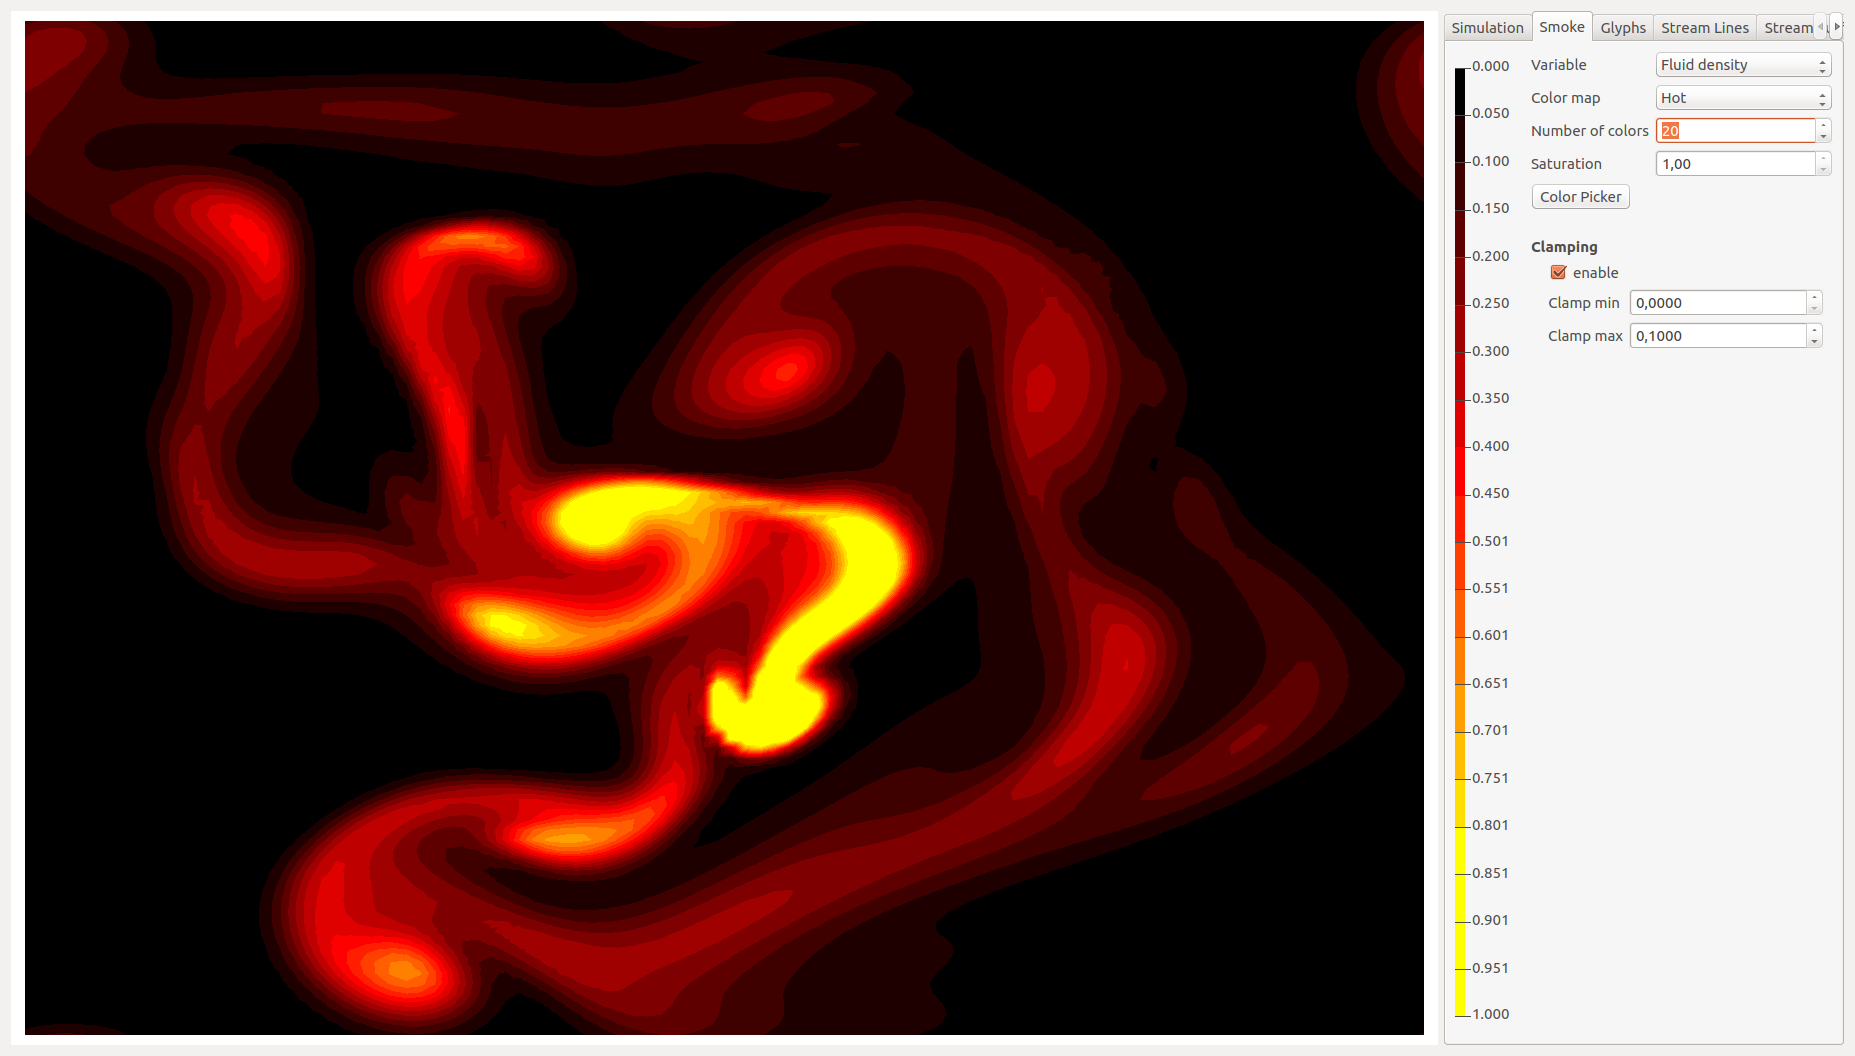
\includegraphics[width=\textwidth, trim={235px 30px 1230px 830px}, clip]{colormapping/img/heat20}
		\caption{Example of a visualization using a heat-map containing 20 colors.}
		\label{fig:colormapping:banding:20}
	\end{subfigure}
	\hspace{50px}
	\begin{subfigure}{0.4\textwidth}
		\centering
		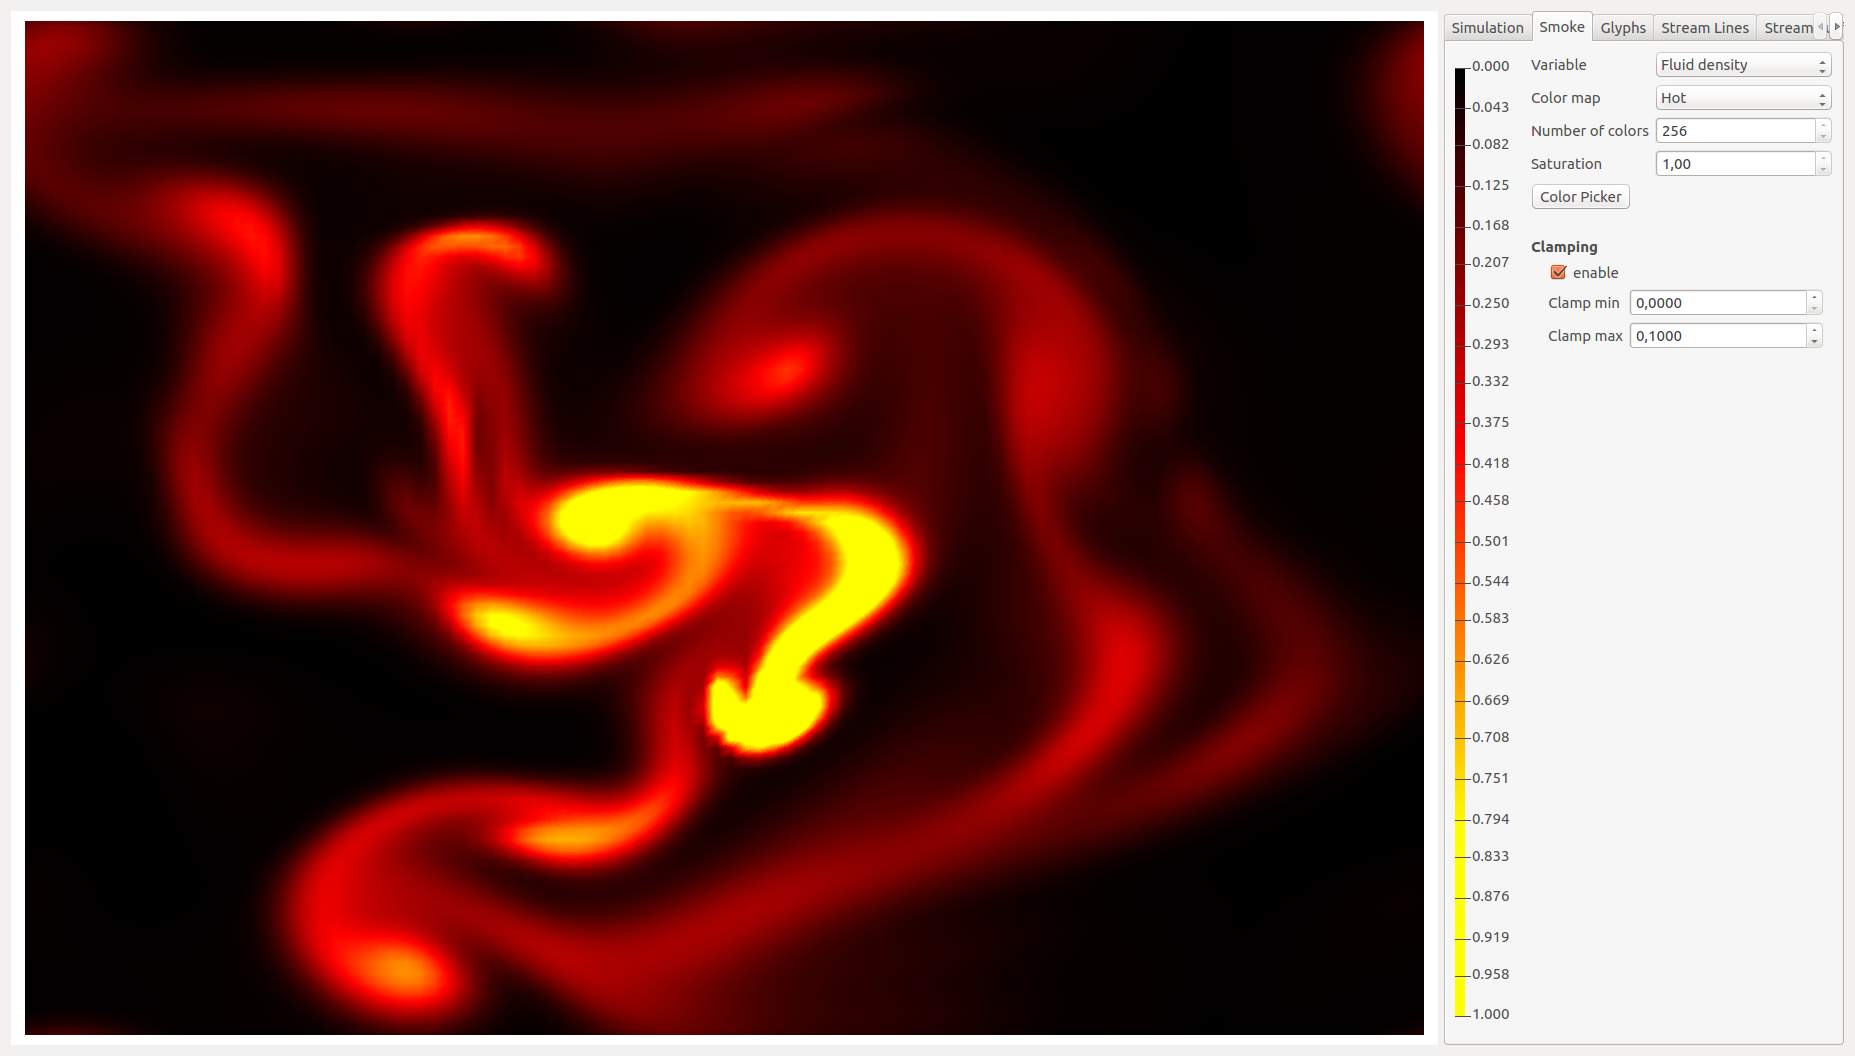
\includegraphics[width=\textwidth, trim={235px 30px 1230px 830px}, clip]{colormapping/img/heat256}
		\caption{Example of a visualization using a heat-map containing 256 colors.}
		\label{fig:colormapping:banding:256}
	\end{subfigure}	
	\caption{The influence of the number of colors in the colormap shown using the heat-map using 20 \subref{fig:colormapping:banding:20} and 256 \subref{fig:colormapping:banding:256} colors. Both images are taken from the same simulation state and zoomed in on the same location to show the effect more clearly.}
	\label{fig:colormaps:banding}
\end{figure}
	\todo[inline]{Number of colors, disadvantages/advantages when to use?}
	\todo[inline]{Change saturation, disadvantages/advantages when to use?}

\subsection{Applying Color Maps}
\label{ss:colormaps:applying}
	\todo[inline]{Discuss clamping}
	\todo[inline]{Discuss scaling}

\subsection{Variables that the Color Maps are Applied to}
\label{ss:colormaps:variables}
	\todo[inline]{Discuss fluid density, what is it? suitable for colormapping? Which colormap?}
	\todo[inline]{Discuss fluid velocity magnitude what is it? suitable for colormapping? Which colormap?}
	\todo[inline]{Discuss force field magnitude what is it? suitable for colormapping? Which colormap?}